\documentclass[a4paper]{article}

\usepackage[english]{babel}
\usepackage{amsmath}
\usepackage{graphicx}

\author{Maarten de Jonge}
\date{\today}
\title{Concurrency and Parallel Programming \\
\large{Test results on DAS-4}}

\begin{document}
\maketitle

\section*{Experimental setup}
The wave equation has been straightforwardly implemented. When $n_p$ points on the
wave are being simulated on $n_t$ threads, each thread handles a slice of
roughly $\frac{n_p}{n_t}$ points, with some variation due to the division not
being guaranteed to be exact.

The simulation has been run on the DAS-4 computer with various values for each
parameter; The number of simulated points is tested at $1.000, 10.000,
1.000.000, 10.000.000$ (with dots added to increase readability), and each of
the values has been tested with 1, 2, 4, 8 and 16 threads. In each case, a
suitable value for the number of time steps has been selected such that the
total time taken with 1 thread is somewhere around 50 seconds, to allow for
decently accurate benchmarking without getting bored. These values can be seen
in table \ref{table:t}.

\begin{table}[htbp]
    \centering
    \begin{tabular}{|l|l|}
        \hline
        number of points & number of iterations \\
        \hline
        $10^3$ & $1e6$ \\
        $10^4$ & $5e5$ \\
        $10^6$ & $5e3$ \\
        $10^7$ & $5e2$ \\
        \hline
    \end{tabular}
    \caption{The number of points with their chosen number of timesteps}
    \label{table:t}
\end{table}

\section*{Results}
\begin{figure}[htbp]
    \centering
    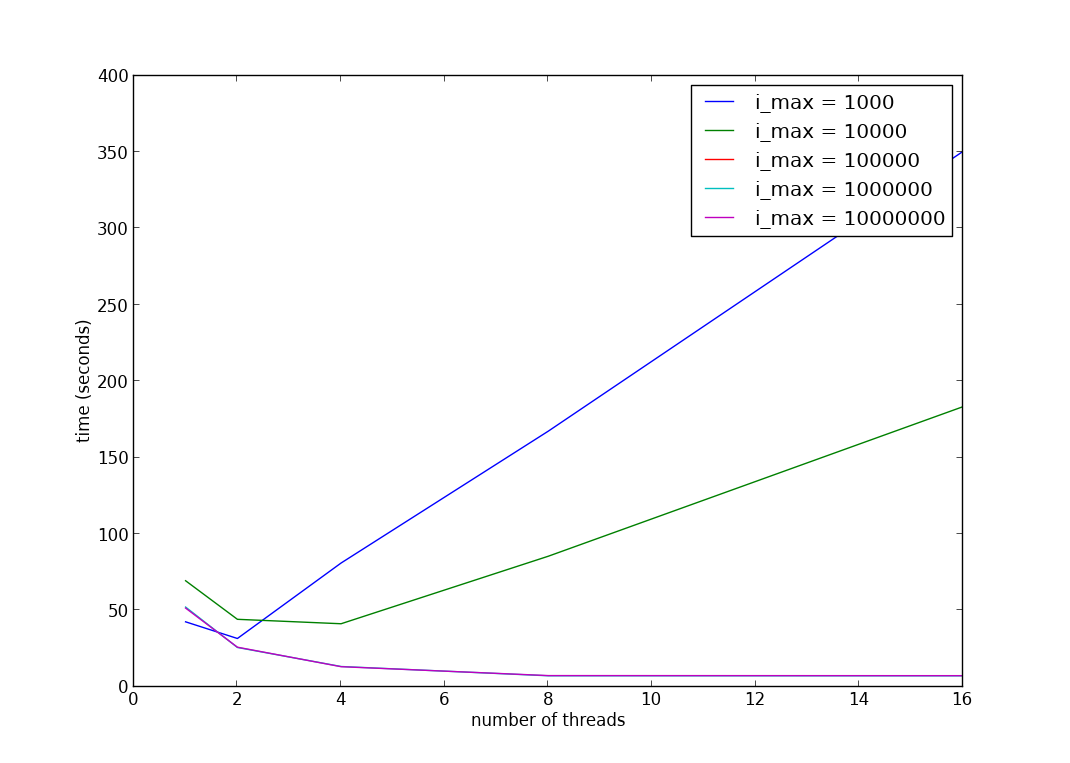
\includegraphics[width=\textwidth]{results.png}
    \caption{The test results. "i\_max" refers to the amount of points
    simulated on the wave.}
    \label{fig:results}
\end{figure}

\begin{table}[htbp]
    \centering
    \begin{tabular}{|l|l|l|l|l|}
        \hline
        i\_max    & t\_max   & num\_threads & time    & normalized \\
        \hline
        1000     & 1000000 & 1           & 42.4294 & $4.24294e-08$ \\
        1000     & 1000000 & 2           & 31.5108 & $3.15108e-08$ \\
        1000     & 1000000 & 4           & 80.9137 & $8.09137e-08$ \\
        1000     & 1000000 & 8           & 167.284 & $1.67284e-07$ \\
        1000     & 1000000 & 16          & 350.395 & $3.50395e-07$ \\
        10000    & 500000  & 1           & 69.3228 & $9.83256e-08$ \\
        10000    & 500000  & 2           & 44.066  &  $6.2502e-08$ \\
        10000    & 500000  & 4           & 41.1647 & $5.83869e-08$ \\
        10000    & 500000  & 8           & 85.3845 & $1.21107e-07$ \\
        10000    & 500000  & 16          & 183.268 & $2.59943e-07$ \\
        1000000  & 5000    & 1           & 52.108  & $7.39086e-08$ \\
        1000000  & 5000    & 2           & 25.6232 & $3.63433e-08$ \\
        1000000  & 5000    & 4           & 13.1806 & $1.86951e-08$ \\
        1000000  & 5000    & 8           & 7.08639 & $1.00511e-08$ \\
        1000000  & 5000    & 16          & 7.06076 & $1.00148e-08$ \\
        10000000 & 500     & 1           & 51.4277 & $7.29436e-08$ \\
        10000000 & 500     & 2           & 25.8168 & $3.66179e-08$ \\
        10000000 & 500     & 4           & 13.0537 & $1.85151e-08$ \\
        10000000 & 500     & 8           & 7.21982 & $1.02404e-08$ \\
        10000000 & 500     & 16          & 7.16489 & $1.01625e-08$ \\
        \hline
    \end{tabular}
    \caption{The raw test data, where ``i\_max'' is the number of simulated points
    on the wave and ``t\_max'' is the amount of iterations.}
    \label{table:results}
\end{table}

Figure \ref{fig:results} shows the results. When simulating 1000 or 10000
points, there is an initial speedup when increasing the amount of threads, but
after a certain point any additional threads will dramatically lower
performance. The higher amounts of points scale very well with the amount of
threads, up to 8 threads (which is the amount of cores available on system).
Scaling it up to 16 threads does not noticably improve performance, although it
doesn't degrade it either. 

\section*{Conclusion}
There appears to be some overheard to the use of threads; they can offer a
significant speedup for the tested scenario, but only when each thread has a
high enough workload. It seems that when there's too little data to simulate per
thread, the work done by the thread will not be worth the incurred overhead,
leading to a (quite severe) degradation of performance.

\end{document}
